\chapter{Revisão de Literatura}
\label{chap:revisao}

Este capítulo trata sobre o processo de revisão de literatura deste trabalho. O procedimento adotado será a Revisão Rápida. Este tipo de revisão é mais adequada para ambientes práticos, ou que necessitam de uma tomada de decisão mais célere, por ter um prazo mais encurtado. Apesar de serem mais simplificadas, os resultados das revisões rápidas e das revisões sistemáticas, apesar de apresentarem divergências, são abordagens que possuem semelhanças nos seus resultados obtidos. A área de Engenharia de Software também tem adotado essa abordagem por conta dessas características \cite{cartaxo2020}:

\begin{itemize}
    \item \textbf{Escopo mais limitado}: são limitadas a problemas práticos e conduzidos no contexto dos profissionais;
    \item \textbf{Metodologia simplificada}: utiliza-se uma quantidade menor de bases bibliográficas, além de limitar a faixa de período das publicações;
    \item \textbf{Necessidade menor de pessoas envolvidas}: as revisões rápidas podem funcionar com a participação de pelo menos uma pessoa;
    \item \textbf{Tempo e custo reduzido}: os dados são trabalhados de uma maneira mais prática, e isso gera um menor tempo e custo do processo de pesquisa, extração e análise dos dados;
    \item \textbf{Maior participação dos profissionais}: como é do caráter da revisão rápida os prolemas práticos dos profissionais, elas exigem uma estreita colaboração com estes.
\end{itemize}

\section{Protocolo de Revisão}
\textbf{Título:} Protocolo de Revisão Rápida sobre os mecanismos da prática da Inovação Social entre a Universidade e a Sociedade

\par\vspace{3\baselineskip}

\textbf{Objetivos da Revisão}
\begin{itemize}
    \item Examinar processos e estruturas que estabelecem a colaboração entre a universidade e a sociedade, buscando identificar as principais práticas colaborativas existentes;
    \item Identificar a forma que a universidade apoia e incentiva a prática da Inovação Social Aberta, explorando os recursos utilizados para essa prática;
    \item Avaliar a atuação da extensão universitária na colaboração entre a universidade e a sociedade, considerando atividades, projetos e impactos gerados por meio dessas práticas;
    \item Sintetizar os resultados das pesquisas existentes para mapear lacunas e dificuldades nas iniciativas de Inovação Social Aberta através da extensão universitária.
    \par\vspace{1\baselineskip}
\end{itemize}

\textbf{Perguntas para revisão}
\begin{itemize}
    \item P1: como a universidade auxilia na prática da inovação social?
    \item P2: qual o mecanismo de colaboração entre a universidade e a sociedade? \cite{brunswicker2018}
    \item P3: como a extensão universitária faz parte dessa colaboração?
    \item P4: quais as evidências e dificuldades acerca da extensão universitária nesse processo? 
\end{itemize}

\section{Estratégias de busca}
A busca foi realizada nas principais bases de dados relevantes científica e academicamente da área de ciência da computação. Os passos de busca foram os seguintes:
\begin{enumerate}
    \item Elaboração das perguntas de pesquisa;
    \item Elaboração de \textit{string} adequada, com sinônimos e traduções para o inglês, para abarcar o máximo de artigos possíveis;
    \item Buscas utilizando aspas (“) nos termos, para filtrar somente os termos exatos e evitar temas não relacionados;
    \item Utilização do termo “\textit{AND}” para alcançar um maior espectro de artigos apresentados com relevância para a pesquisa;
    \item Estudos publicados até 6 anos (2017–2023), para considerar um limiar de tempo maior em decorrência da pandemia ocorrida no ano de 2019. 
\end{enumerate}

\textbf{\textit{Strings} de busca}

Para alcançar um maior quantitativo de artigos, foi realizada a busca em dois idiomas: português, o idioma nativo desta pesquisa e o inglês.
\begin{quadro}[H]
\centering
\caption{Termos utilizados na busca}
\begin{tabular}{|c|c|}
\hline
\rowcolor[HTML]{C0C0C0} 
\textbf{Termos Originais} & \textbf{Traduções} \\ \hline
Inovação Social           & Social Innovation  \\ \hline
Universidade              & University         \\ \hline
\end{tabular}
\newline
\newline
Fonte: O autor (2024).
\end{quadro}



Resultando na string de busca abaixo, utilizando os passos citados anteriormente:

\begin{quadro}[H]
\centering
\caption {\textit{Strings} de busca}
\begin{tabular}{|c|c|c|}
\hline
\rowcolor[HTML]{C0C0C0} 
\textbf{Termo 1} & \textbf{Operador} & \textbf{Termo 2}    \\ \hline
"\textit{UNIVERSITY}"     & \textit{AND}               & "\textit{SOCIAL INNOVATION}" \\ \hline
"UNIVERSIDADE"   & \textit{AND}               & "INOVAÇÃO SOCIAL"   \\ \hline
\end{tabular}
Fonte: O autor (2024).
\end{quadro}


\textbf{Bases de dados utilizadas}

As bases de dados utilizadas são as bases mais conhecidas e conceituadas na área da Ciência da Computação e de áreas correlatas.

\begin{quadro}[H]
\caption{Bases de dados utilizadas}
\centering
\begin{tabular}{|c|c|}
\hline
\rowcolor[HTML]{C0C0C0} 
\textbf{Base de dados}                                     & \textbf{Endereço} \\ \hline
IEEE — Instituto de Engenheiros Eletricistas e Eletrônicos & ieee.org          \\ \hline
SBC \textit{Open Library} — Sociedade Brasileira de Computação      & sol.sbc.org       \\ \hline
\end{tabular}
\newline
\newline
Fonte: O autor (2024).
\end{quadro}




Uma das principais bases de dados da área da computação, a \textit{\gls{ACM} Digital Library}, apresentou um resultado de 320 artigos, porém, em decorrência da \gls{CAPES} não proporcionar o acesso gratuito a esta base de dados, a sua utilização foi descartada nessa revisão.


\textbf{Justificativa de escolha das bases}
\begin{itemize}
    \item \textbf{IEEE — Instituto de Engenheiros Eletricistas e Eletrônicos}: É um dos principais institutos de pesquisa científica do mundo na área de tecnologia e engenharia;
    \item \textbf{SBC \textit{Open Library} — Sociedade Brasileira de Computação}: é a revista da \gls{SBC}, referência na área da computação no país, além de uma das principais responsáveis junto ao Ministério da Educação na elaboração de currículo dos cursos de graduação na área.
\end{itemize}


\section{Busca automática}
Inicialmente, foi realizada uma busca automática seguindo os critérios determinados anteriormente, filtrando pelas bases de dados já listadas e pelo período de 2017 a 2023, foram retornados um total de 251 trabalhos. A base SBC \textit{Open Library}, não retornou nenhum artigo, tanto em buscas por termos em português como em termos em inglês, como mostra a tabela abaixo: 

\begin{table}[H]
\centering
\caption{Quantidade de estudos localizados}
\begin{tabular}{p{10cm}c}
\rowcolor[HTML]{C0C0C0} 
\textbf{Base de dados} & \textbf{Quantidade de artigos} \\
\hline
IEEE — Instituto de Engenheiros Eletricistas e Eletrônicos & 251 \\
SBC \textit{Open Library} — Sociedade Brasileira de Computação & 0 \\
\rowcolor[HTML]{C0C0C0} 
\textbf{Quantidade total} & \textbf{251} \\
\end{tabular}
\vspace{0.2cm}
Fonte: O autor (2024).
\end{table}


Ao observar o ano de publicação, observa-se que o ano de 2022 apresentou uma tendência de publicação maior que nos outros anos,  demonstrando uma retomada de estudos que haviam sido paralisados em decorrência da pandemia de COVID-19.

\begin{figure}[H]
    \centering
    \caption{Número de estudos publicados por ano}
    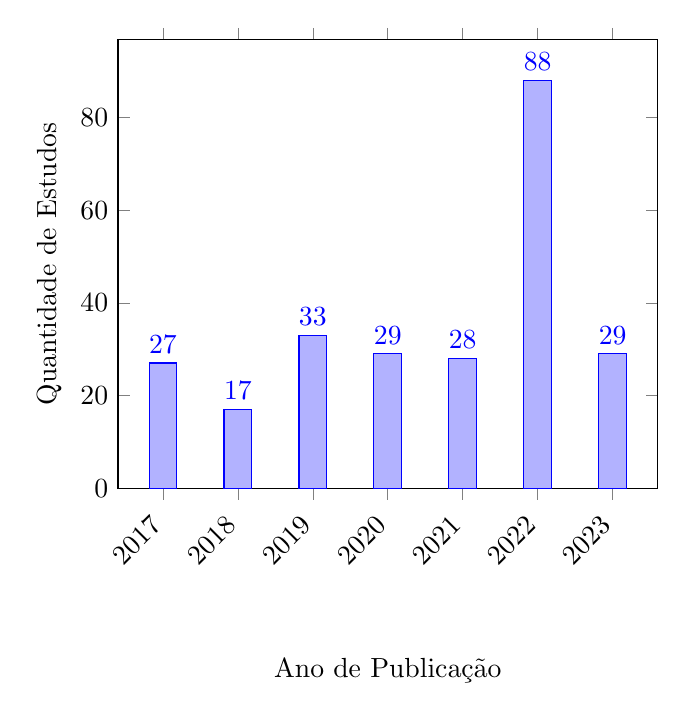
\begin{tikzpicture}
        \begin{axis}[
            ybar,
            symbolic x coords={2017, 2018, 2019, 2020, 2021, 2022, 2023},
            xtick=data,
            ymin=0,
            ylabel={Quantidade de Estudos},
            xlabel={Ano de Publicação},
            xlabel style={yshift=-25pt}, % Move o rótulo do eixo X para baixo
            nodes near coords,
            bar width=10pt, % Aumenta a largura das barras
            enlarge x limits=0.1, % Aumenta o espaçamento entre as barras
            xticklabel style={yshift=-5pt, rotate=45, anchor=east} % Rotaciona e desloca os rótulos do eixo X
        ]
        \addplot coordinates {(2017,27) (2018,17) (2019,33) (2020,29) (2021,28) (2022,88) (2023,29)};
        \end{axis}
    \end{tikzpicture}
    \\
        \centering Fonte: O autor (2024).
\end{figure}


\section{Escolha dos estudos}

Inicialmente foi realizada uma seleção preliminar analisando o título e resumos dos artigos, excluindo inicialmente estudos que não haviam relação com a temática proposta na revisão, resultando em 79 potenciais estudos a serem analisados. Após essa etapa preliminar, foi realizada a filtragem através dos Critérios de Inclusão e Exclusão citados abaixo.

\par\vspace{1\baselineskip}

\textbf{Critérios de inclusão}
\begin{itemize}
    \item CI-1: Pesquisas que tratam da inovação social aberta;
    \item CI-2: Pesquisas que tragam práticas realizadas por meio de universidades;
    \item CI-3: Pesquisas que são estudos primários.
\end{itemize}

\par\vspace{1\baselineskip}

\textbf{Critérios de exclusão}
\begin{itemize}
    \item CE-1: Pesquisas que não tratam do tema da inovação social aberta;
    \item CE-2: Pesquisas que não tenham sido realizadas no âmbito universitário;
    \item CE-3: Pesquisas que não são estudos primários (Resumos, resenhas, apresentações, e afins).
\end{itemize}

Dentre os 79 pré-selecionados, 22 foram removidos por serem não-primários (CE-3), e 46 por não tratarem da temática de inovação social aberta (CE-1) e/ou por não serem realizados no âmbito universitário (CE-2). 

O total de artigos que atenderam os três critérios de inclusão foi de 11 artigos.

\begin{table}[H]
\centering
\caption{Apresentação do quantitativo de estudos totais e selecionados}
\begin{tabular}{cccc}
\rowcolor[HTML]{C0C0C0} 
\textbf{Base de dados} & \textbf{Total} & \textbf{Selecionado} & \textbf{\%} \\
IEEE                   & 251            & 11                   & 4,38\%      \\
SBC/SOL                & 0              & 0                    & 0\%        
\end{tabular}
\vspace{0.2cm}

{\centering Fonte: O autor (2024). \par}
\end{table}




Os artigos foram publicados por pesquisadores de universidades dos seguintes países: EUA, Portugal e Tailândia com dois artigos cada e Africa do Sul, Brasil, China, Noruega, Sri Lanka, e Taiwan, possuem somente um artigo cada.

\section{Direcionamento dos Artigos}

Ao realizar uma leitura profunda e observação de cada um dos artigos, é possível observar através de seus objetivos, o direcionamento de cada artigo, como demonstrado na tabela abaixo.

\begin{table}[H]
\centering
\caption{Classificação dos estudos}
\begin{tabular}{cc}
\rowcolor[HTML]{C0C0C0} 
\textbf{Classificação}  & \textbf{Quantidade} \\
Relato de experiência   & 7                   \\
Proposta de metodologia & 4                   
\end{tabular}
\vspace{0.2cm}

{\centering Fonte: O autor (2024). \par}
\end{table}


\section{Resposta as perguntas da Revisão}

Para facilitar a compreensão do atual panorama da literatura, essa subseção irá apresentar a resposta para as perguntas da revisão, conforme os artigos selecionados.

\subsection{P1: como a universidade auxilia na prática da Inovação Social Aberta?}

Todos os artigos selecionados tratam da forma a qual a universidade realiza práticas de inovação social. O artigo S001 relata que a Universidade praticou a inovação social através da Aprendizagem de Serviço, que combina serviço comunitário voluntário e o aprendizado acadêmico, possibilitando a exploração de problemas existentes na comunidade e sua resolução através da experiência acadêmica, unindo a teoria e a prática. 

O artigo S003 utilizou a Filosofia da Economia de Suficiência (SEP), um modelo de desenvolvimento sustentável através da autossuficiência, capacitando a comunidade para atuação, auxiliando a identificação dos problemas e os dados, e a implementação de soluções viáveis pela própria comunidade. 

Já os artigos S002, S004, S007, S008 e S009 também trazem a dinâmica da universidade fornecendo capital humano e/ou material, pesquisa e desenvolvimento, suporte técnico, capacitação e formação de competências. Já os artigos S006 e S010 relatam construir soluções por parcerias entre as universidades, empresas e órgãos governamentais.  

No artigo S011, as práticas inovativas sociais ocorrem através do ensino ativo, que coloca os estudantes no centro do processo de aprendizado, estimulando também a interação entre estes e os grupos vulneráveis que irão realizar a inovação social, de fato. 

O artigo S005 evidencia a Universidade fornecendo \textit{frameworks} que promovem a criação de soluções para problemas urbanos colaborativamente entre a universidade, a administração pública e os cidadãos.

A análise dos artigos revela que, geralmente, a universidade atua como principal força motriz da realização da Inovação Social, e agindo como uma capacitadora, realizando a Inovação Aberta de dentro para fora, como pontuado por Chesbrough 2014), uma inovação que a organização abre seu processo para servir de entrada para outras organizações, praticando de forma tímida a inovação aberta de fora para dentro, onde no caso, a Universidade receberia \textit{inputs} da comunidade onde está atuando e a inovação acoplada, onde a cocriação, como um de seus principais métodos, permitiria que a criação de soluções em conjunto entre a comunidade e a universidade. 

Outro cenário observado é onde a universidade atua através parcerias com instituições, órgãos governamentais e afins, não proporcionando em sua plenitude as criações colaborativas através da Inovação Aberta acoplada. O cenário da prática da inovação social aberta em sua plenitude, através do processo de fato colaborativo, demonstrando assim, que a prática da Inovação Social Aberta encontra-se pouco difundida na academia. Os números podem ser verificados na sumarização na tabela abaixo:

\begin{table}[H]
\centering
\caption{Classificação quanto à forma da prática da Inovação Social Aberta}
\begin{tabular}{ccc}
\rowcolor[HTML]{C0C0C0} 
\textbf{Classificação}  & \textbf{Artigos}             & \textbf{Quantidade} \\
Universidade "facilitadora"  &  \begin{tabular}[c]{@{}c@{}}S002, S004, S007\\  S008, S009\end{tabular} & 5                   \\
Processos colaborativos & S001, S003, S005, S011       & 4                   \\
Parcerias entre órgãos  & S006, S010                   & 2                   
\end{tabular}
\vspace{0.2cm}

{\centering Fonte: O autor (2024). \par}
\end{table}



\subsection{P2: quais os mecanismos de colaboração entre a universidade e a sociedade?} \cite{brunswicker2018}

O artigo S001 destaca o mecanismo de colaboração entre a universidade, empresas e a comunidade, no qual os alunos atuaram diretamente com as empresas patrocinadoras e as organizações comunitárias. Semelhantemente, o artigo S002 aborda a cocriação de um \textit{Makerspace}, um espaço dedicado à cultura criativa e o desenvolvimento colaborativo. 

O artigo S003 descreve a criação de um curso pela Universidade que permite a interação direta entre alunos, facilitadores e \textit{stakeholders} externos. Da mesma forma, o artigo S010 apresenta a criação de Laboratórios de Vivência Urbana, onde a comunidade, a universidade e o governo trabalham em conjunto na cocriação de soluções urbanas segundo a necessidade da sociedade. 

Os artigos S004, S005, S006 e S007, S008, S009 E S011 enfatizam criar ecossistemas colaborativos mediante parcerias com empresas, órgãos públicos e a comunidade. 

O cenário se assemelha às conclusões da P1. Seguindo o conceito de modelos de inovação aberta de \citeauthor{brunswicker2018} (\citeyear{brunswicker2018}), é possível notar que a Universidade atua majoritariamente por meio de parcerias, para a colaboração. As principais iniciativas que representam a totalidade da Inovação Aberta tratam da criação de laboratórios e espaços de vivência, onde a universidade, a sociedade e o governo podem pensar e cocriar inovações e soluções. Além disso, existe um caso de criação de cursos que promovem a Inovação Social Aberta. Os números podem ser verificados na sumarização na tabela abaixo:
 

\begin{table}[H]
\centering
\caption{Classificação quanto aos mecanismos de colaboração universidade/sociedade}
\begin{tabular}{ccc}
\rowcolor[HTML]{C0C0C0} 
\textbf{Classificação}                                                              & \textbf{Artigos}                             & \textbf{Quantidade} \\
\begin{tabular}[c]{@{}c@{}}Parcerias bilaterais\\\end{tabular} & \begin{tabular}[c]{@{}c@{}}S001, S003, S004, S006 \\ S009, S010\end{tabular} & 8                   \\
Concursos e torneios                                                                  & S005, S008                                                                               & 2                   \\
Comunidades e redes                                                                & S008, S011                                                                               & 2                   \\
Intermediários de inovação                                                                 & S007                                                                                     & 1                  
\end{tabular}

\vspace{0.2cm}

{\centering Fonte: O autor (2024). \par}
\end{table}



\subsection{P3: como a extensão universitária faz parte dessa colaboração?}

A cultura de extensão universitária é algo que pode variar de país para país. Esse conceito é muito característico das universidades brasileiras, e pode ser chamado por outros nomes em outros países, como \textit{University Outreach}. Dos 11 artigos, somente um é brasileiro. Apesar da extensão não ser mencionada, as atividades de todos os artigos selecionados possuem a natureza extensionista de colaboração, que se materializa na troca de saberes entre universidade e sociedade (através da interação dialógica), além do impacto gerado na formação do estudante e também na sociedade.


\subsection{P4: quais as evidências e dificuldades acerca da extensão universitária nesse processo?}

O artigo S001 destaca como principais pontos melhoria: maior desempenho acadêmico dos alunos, desenvolvimento de habilidades e criação de conexões com empregadores, porém, aponta como desafios a necessidade de financiamento, dificuldade no engajamento de parceiros a longo prazo, e dependência de apoio contínuo para prosseguimento do projeto. Da mesma forma, o artigo S002 menciona como pontos positivos: aumento da confiança dos participantes, desenvolvimento de habilidades técnicas e mudança de percepção sobre a capacidade dos participantes. Os desafios foram a manutenção do engajamento, superação das barreiras sociais e sustentabilidade financeira do projeto. 

O artigo S003 ressalta o sucesso no novo sistema de abastecimento de água, que teve seu êxito em decorrência do envolvimento e colaboração entre universidade, governo e comunidade, e destaca como dificuldades a necessidade de manutenção contínua e sustentabilidade financeira do projeto. Já o artigo S004 aponta que a abordagem utilizada melhorou o engajamento e criatividade dos participantes, porém, enfrentou como dificuldades a limitação de tempo para a colaboração, dificuldades no uso das plataformas digital e problemas de envolvimento dos stakeholders. O artigo S005 apresenta como pontos positivos o envolvimento acadêmico, mas aponta como desafio a motivação da participação contínua dos cidadãos. 

No contexto do desenvolvimento profissional, o artigo S006 apresenta como pontos positivos o desenvolvimento da indústria local e capacitação dos profissionais, porém, aponta como dificuldades a falta de tecnologia para os trabalhadores locais. O artigo S007 cita que os principais desafios foram a falta de colaboração entre a universidade e a sociedade. Já o artigo S008 menciona o financiamento do projeto e sua viabilidade econômica como seus principais desafios.

Os artigos S009 e S010 tratam de questões sobre comunicação e implementação dos projetos. O artigo S009 destaca as dificuldades de comunicação e colaboração entre a universidade e as empresas, pois, a pesquisa acadêmica muitas vezes não é facilmente compreendida pelas empresas. Também é mencionada as dificuldades de financiamento do projeto e resistência a mudança dos \textit{stakeholders} citados no artigo. Já o artigo S010 ressalta como dificuldades a necessidade de adaptação das metodologias acadêmicas para o contexto prático, a dificuldade do engajamento contínuo e a dependência de financiamento.

O artigo S011 destaca como melhorias: aumento da motivação e criação da inovação. No entanto, menciona como desafios a adaptação das metodologias acadêmicas para o contexto prático, além da dependência de financiamento. 

É possível observar que, na maioria nos artigos, a dificuldade é da sustentabilidade financeira do projeto, pois, em decorrência dos projetos serem realizados no âmbito universitário, necessitam de investimentos externos a universidade. Em seguida, é o envolvimento/engajamento dos participantes. Outro ponto relatado em diversos artigos, é a facilitação dos conteúdos acadêmicos para o contexto prático, com atores fora da academia e também a resistência a mudança de alguns setores da sociedade com as inovações propostas e construídas. Um artigo relatou como dificuldade a falta da comunicação entre as partes envolvidas no projeto. Os números podem ser verificados na sumarização na tabela abaixo:


\begin{table}[H]
\centering
\caption{Classificação conforme as evidências e dificuldades relacionadas à extensão universitária}
\begin{tabular}{ccc}
\rowcolor[HTML]{C0C0C0} 
\textbf{Classificação}                                                       & \textbf{Artigos}                       & \textbf{Quantidade} \\
\begin{tabular}[c]{@{}c@{}}Sustentabilidade\\ financeira\end{tabular}        & \begin{tabular}[c]{@{}c@{}}S001, S002, S003, S008,\\ S009, S010, S011\end{tabular} & 7                   \\
\begin{tabular}[c]{@{}c@{}}Dificuldades de\\ engajamento\end{tabular}        & \begin{tabular}[c]{@{}c@{}}S001, S002, S004,\\  S005, S009, S010\end{tabular}      & 6                   \\
\begin{tabular}[c]{@{}c@{}}Adaptação\\ dos métodos\\ acadêmicos\end{tabular} & S010, S011                                                                         & 2                   \\
\begin{tabular}[c]{@{}c@{}}Resistência a\\ mudança\end{tabular}              & S009, S010                                                                         & 2                   \\
\begin{tabular}[c]{@{}c@{}}Problemas de\\ comunicação\end{tabular}           & S007                                                                               & 1                   
\end{tabular}
\vspace{0.2cm}

{\centering Fonte: O autor (2024). \par}
\end{table}


\section{Considerações finais da Revisão}

O quantitativo de artigos demonstra a carência da literatura acerca do trabalho da Inovação Social Aberta praticada no âmbito das universidades, e justifica a necessidade deste trabalho. O quantitativo de artigos publicados por brasileiros demonstra que este tema aparenta ser pouco explorado pela academia no país. As perguntas também pontuam que as maiores dificuldades nos projetos de Inovação Social Aberta são a falta de investimento, a dificuldade no engajamento das partes e resistência a mudança por parte dos setores da sociedade. E que os ganhos das práticas são benéficos tanto para a sociedade, que possui seu problema solucionado, quanto para a universidade, que consegue estreitar os laços com a sociedade, além de preparar melhor seus estudantes para a resolução de problemas. Os artigos selecionados demonstram as formas de colaboração existentes entre a universidade e a sociedade, e quais são os principais êxitos e dificuldades que foram encontradas ao longo deste processo colaborativo, mostrando também a forma que a universidade apoia e incentiva estas práticas de Inovação Social Aberta, além dos impactos gerados pelas mesmas.